\subsection*{Visitors} \label{sec:visitors}
% The top-down and bottom-up force computation presented in Section~\ref{sec:mappings} is easily generalized to an arbitrarily branched hierarchy with forces applied at all levels.
We implement the simulation using visitors which traverse the scene top-down and bottom-up, and call the corresponding virtual functions at each graph node traversal. 
A possible implementation of the traversal of a tree-like graph is shown in the left of Figure~\ref{fig:visitorTraversal}.
Algorithmic operations on the simulated objects are implemented by deriving the Visitor class and overloading its virtual functions \textit{topDown(~)} and \textit{bottomUp(~)}. 
This approach hides the scene structure (parent, children) from the components, for more implementation flexibility and a better control of the execution model.
The data structure can easily be generalized from strict hierarchies to directed acyclic graphs for more general kinematic dependencies.
Moreover, various parallelism strategies can be applied independently of the mechanical computations performed at each node.
\begin{figure}
\begin{center}
\begin{tabular}{l|r}
\begin{minipage}{0.4\linewidth}
\begin{algorithmic}
\STATE void  \textbf{Visitor::traverse(Node n)}
\STATE bool continue = this.topDown( n )
\IF{continue} 
\FORALL {c child of n} 
\STATE traverse( c ) 
\ENDFOR
\STATE     this.bottomUp( n )
\ENDIF
\end{algorithmic} 
\end{minipage}
 &
\begin{minipage}{0.5\linewidth}
\begin{algorithmic}
% \renewcommand{\algorithmicendfor}{}
% \renewcommand{\algorithmicendif}{}
\STATE bool  \textbf{AnimateVisitor::topDown(Node n)}
\IF{masterSolver} 
\STATE masterSolver.animate(this.dt)
\RETURN false
\ENDIF
\IF{collisionPipeline} 
\STATE collisionPipeline.modelContacts()
\ENDIF
\IF{odeSolver} 
\STATE odeSolver.solve(this.dt)
\RETURN false
\ENDIF
\FORALL {InteractionForce f}
\STATE f.apply()
\ENDFOR
\RETURN true
\end{algorithmic} 
\end{minipage}
\end{tabular}
\end{center}
\caption{Left: a recursive implementation of the visitor traversal. Right: the AnimateVisitor. }
\label{fig:visitorTraversal}
\end{figure}

Forward time stepping is implemented using the \textit{AnimateVisitor} traversal method, shown in the right of Figure~\ref{fig:visitorTraversal}.
Applied to the simple scene in Figure~\ref{fig:liver-mechanical-spheres}, it triggers the ODE solver, which in turn applies its algorithm using visitors for mechanical operations such as propagating states through the mappings or accumulating forces.
Note that the traversal of the AnimateVisitor is pruned when a ODE solver is encountered.
This allows the ODE solver to take control of its subgraph and to overload lower-level solvers, which are not reached by the AnimateVisitor.
In the more complex scene shown in Figure~\ref{fig:twoObjects}, the solver triggers the collision detection, which may create a contact between the chidren, such as contactSpring.
The visitor then triggers the computation of the interaction force, which will be seen by the objects as a constant, external force during the time step.
The visitor then continues the traversal and triggers each object ODE solver.
The default behavior is to model the contacts prior to applying time integration.
To implement other strategies, a \textit{MasterSolve}r can be used to prune the visitor and apply time integration and collision detection in a different order, possibly looping until all collisions are solved.

\begin{figure}
 \centering
 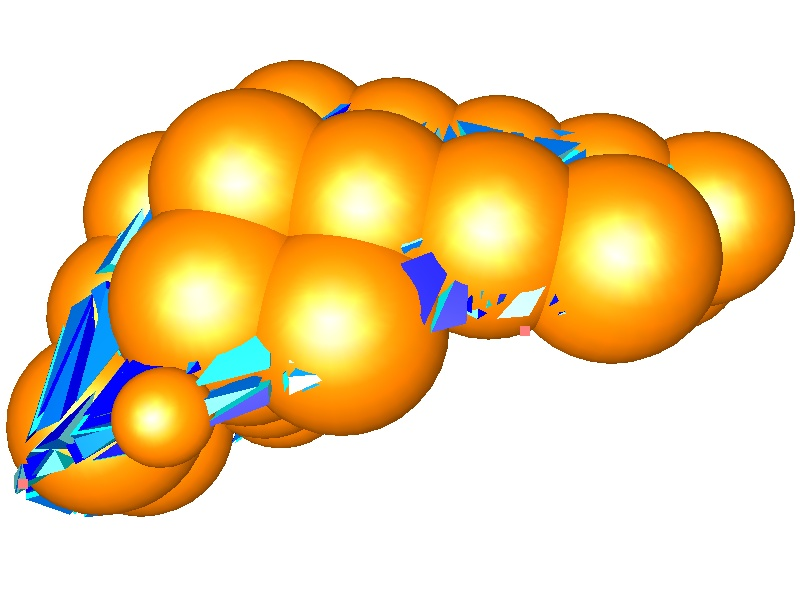
\includegraphics[width=0.4\linewidth]{liver-spheres-superimposed.jpg}
 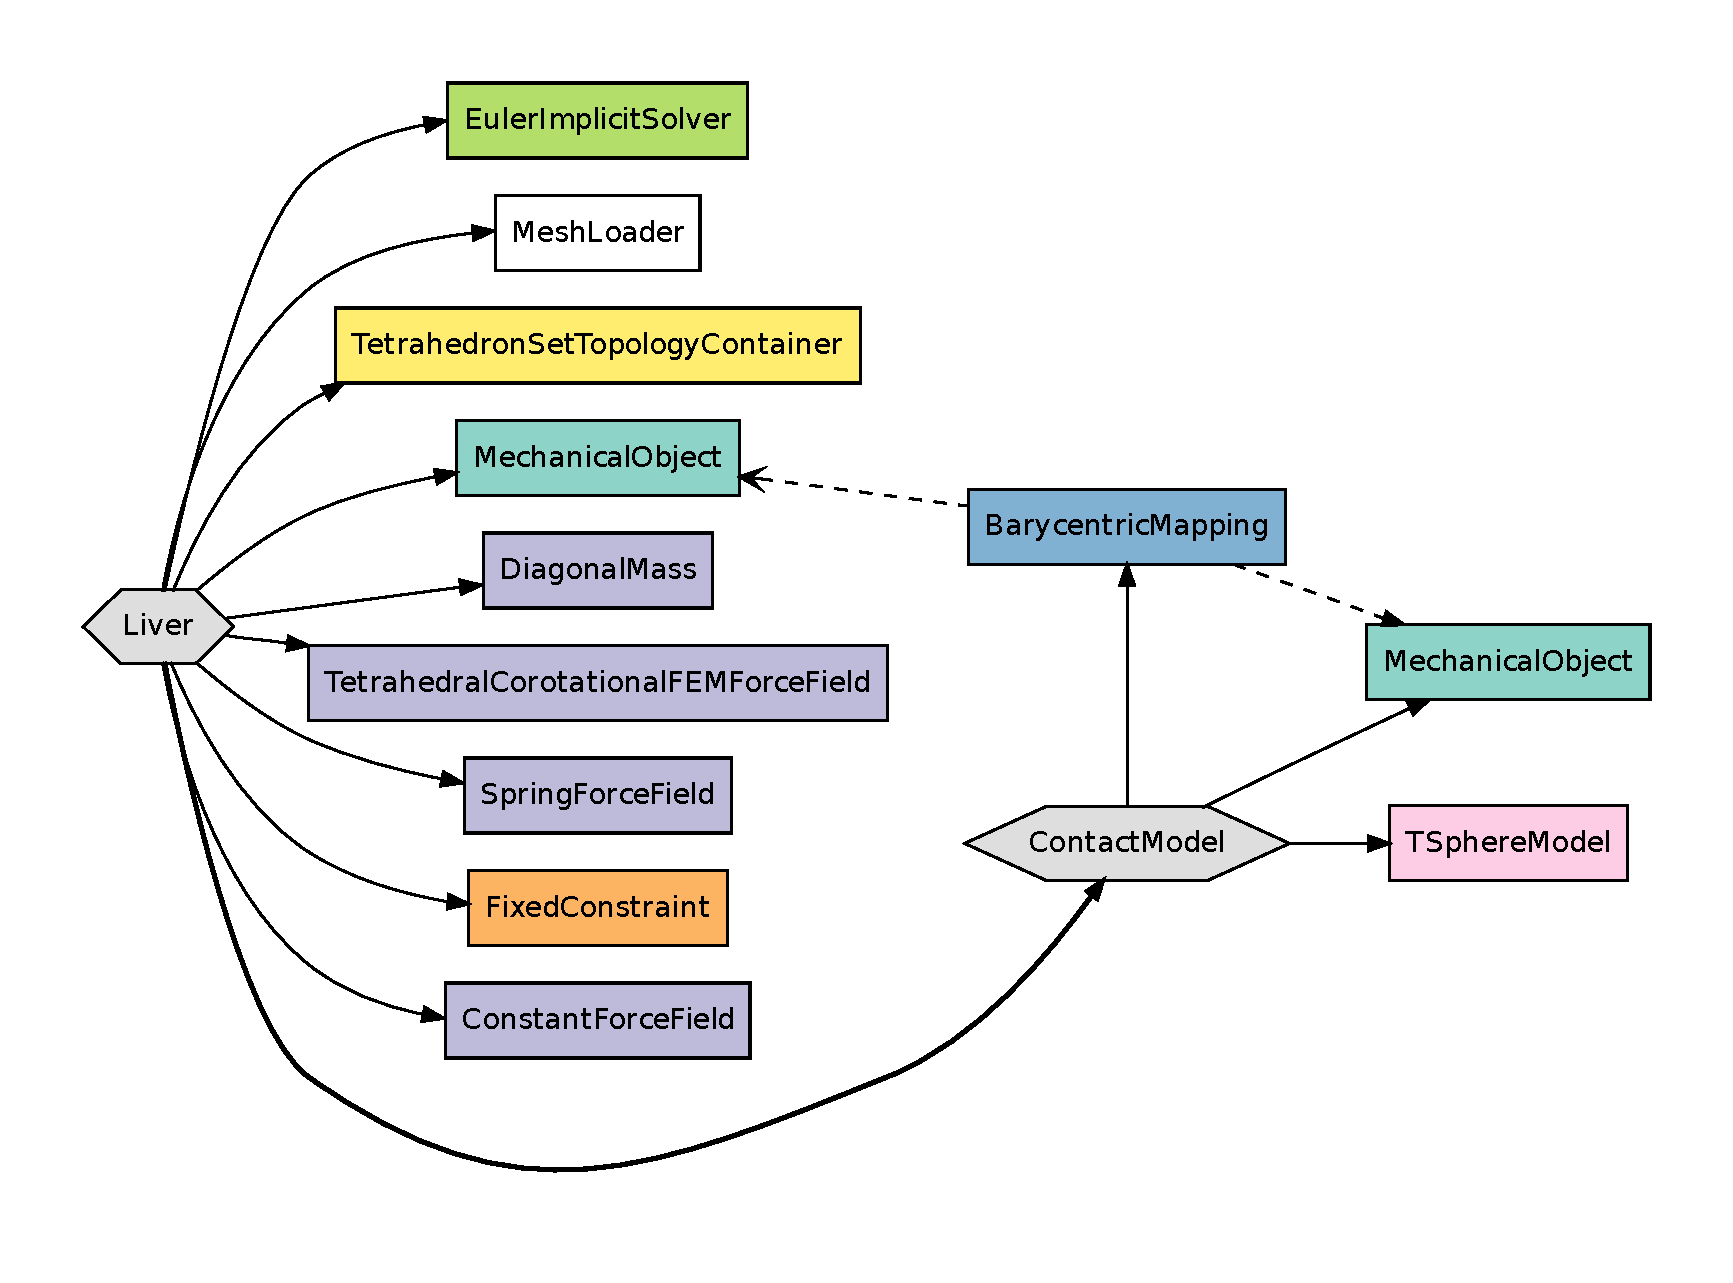
\includegraphics[width=0.56\linewidth]{liver-spheres.pdf}   % generated from ps using: dvipdf -dEPSCrop
 \caption{Left: simple mechanical (in blue) and collision (in yellow) models of a liver. Right: the corresponding scene graph. The plain arrows denote hierarchy, while the stippled arrows represent connections.}
 \label{fig:liver-mechanical-spheres}
\end{figure}

